\documentclass{article}
\usepackage[utf8]{inputenc}
\usepackage{amsmath}
\usepackage[spanish,es-tabla]{babel}
\usepackage{graphicx}
\usepackage{amssymb, amsmath, amsbsy} 
\usepackage{mathtools}
\usepackage{multicol}
\usepackage{scalerel,amsmath}
\usepackage [ spanish ]{babel}
\usepackage [utf 8]{inputenc }
\usepackage {graphicx }
\usepackage[left=1.0cm,top=2.5cm,right=1.0cm,bottom=2.5cm]{geometry}
\title{TP2}

\author{Pablo Herrera - Thomás Mendoza  - Pablo Ramírez}
\date{May 2021}

\begin{document}
	
	\maketitle
	
	\section{Pregunta 1}
	
		\subsection {a)}
	$$
	\max_{{c_{t},n_t,k_t,Q_t,d_t}_t^\infty} E_{0}\sum_{t}^\infty \beta^{t} ln (c_{t}) + \eta (1-e_{t}l_{t})-\dfrac{\kappa}{2}(e_{t}-1)^2l_{t}]
	$$
	Lagrangiano:
	$$
	\mathcal{L}:E_{0}\sum_{t}^\infty \beta^{t}{[\gamma ln c_{t} + \eta (1-e_{t}l_{t})-\dfrac{\kappa}{2}(e_{t}-1)^2l_{t}]+\lambda_{t}[A_t k_t^\alpha (e_tl_t)^{1-\alpha}+d_t-c_t-k_{t+1}+(1-\delta)k_t-d_{t-1}(1+r_{t-1}-\dfrac{\phi(k_{t+1}-k_t)^2}{2})]}	
	$$\\
	CPO  \\
	\begin{equation}
		\mathcal{L}_{c_{t}}: 
		\frac{\gamma}{c_t}= \lambda_t
	\end{equation}
	
	\begin{equation}
		\mathcal{L}_{l_{t}}: 
		\eta e_t+\dfrac{\kappa}{2}(e_{t}-1)^2=\frac{\gamma (1-\alpha)}{c_t} \dfrac{y_t}{l_t}
	\end{equation}
	
	\begin{equation}
		\mathcal{L}_{d_{t}}: 
		\frac{\gamma}{c_t}=\beta (1+r_t)E_t	\frac{\gamma}{c_{t+1}}
	\end{equation}
	
	\begin{equation}
		\mathcal{L}_{k_{t+1}}: 
		\frac{\gamma}{c_t}[1+\phi(k_{t+1}-k_t)]=\beta \frac{\gamma}{c_{t+1}}[\alpha \dfrac{y_{t+1}}{k_{t+1}}+(1-\alpha)+\phi(k_{t+1}-k_t)]
	\end{equation}
	
	\begin{equation}
		\mathcal{L}_{e_{t}}: 
		\eta l_t+\kappa(e_{t}-1)l_t=\frac{\gamma (1-\alpha)}{c_t} \dfrac{y_t}{l_t}
	\end{equation}
	
	\begin{enumerate}
		
		\item  \textbf{Equilibrio del mercado de trabajo:} Bajo la información en t-1, los agentes eligen $l_t$ óptimo del siguiente periodo (esto es equivalente para las firmas).
		$$
		E_{t-1}[\frac {\gamma}{c_t}(1-\alpha)\frac {y_t}{e_t l_t}-\eta]=0
		$$
		
		\item \textbf{Decisión intratemporal}:  Si  la economía no cambia entre lo que es antes conocidos los estados de la naturaleza de la tecnología y la inversión, los agentes elegirán trabajar exactamente lo planeado en el periodo t-1. De lo contrario, estos ajustarán su decisión óptima mediante el esfuerzo.
		$$
		\frac{\gamma}{c_t}(1-\alpha)\frac{y_t}{e_t l_t}-\eta=\frac{\theta(e_t-1)}{l_t}
		$$
		
		\item \textbf{Euler de consumo:} El beneficio marginal esperado de consumir una unidad hoy(dado el shock en la inversión) debe igualar el beneficio marginal de consumir una unidad mañana.
		$$
		\frac{1}{c_t\xi_t}=\beta[\alpha\frac{\gamma}{c_{t+1}}\frac{y_{t+1}}{k_{t+1}}+(1-\delta) \frac{\gamma}{c_{t+1}} \frac{1}{xi_{t+1}}
		$$
		
		
		\item \textbf{Restricción:} El producto debe ser igual al consumo más la inversión.
		$$
		y_t=c_t+i_t
		$$
		
		\item \textbf{Ley de movimiento del capital:}El capital del siguiente periodo se descompone en: capital depreciado del periodo pasado más inversión (esta última sujeto a un shock con proceso estocástico)
		$$
		k_{t+1}=(1-\delta)k_t+\xi_ti_t
		$$
		\item \textbf{Producto}: Función de producción cobb-douglas sujeto a un shock tecnológico (estocástico) . La participación del capital es $\alpha$ y la del trabajo por esfuerzo (1-$\alpha$).
		$$
		y_t=A_t k_t^\alpha (e_tl_t)^{1-\alpha}
		$$
		\item Proceso estocástico del shock tecnológico
		$$
		\ln A_t=\rho \ln A_{t-1}+u_1
		$$
		\item Proceso estocástico del shock en la inversión
		$$
		\ln \xi_t=\rho_\xi \ln \xi_{t-1}+u_2
		$$
	\end{enumerate}
	
	Interpretación de gráficos ante un shock en la tecnología:
	
	\begin{itemize}
		
		\item \textbf{Imagen 1 y 2 (A e Y) :} Tanto el producto como la fuente del shock (A) aumentan de manera proporcional al valor de este mismo, dada la función de producción. A medida que pasan más periodos, el shock converge a su media 0 y el producto y la tecnología vuelven a su estado estacionario.
		\begin{figure}[h]
			\centering
			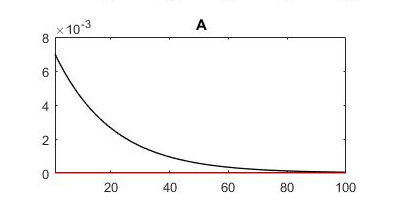
\includegraphics[width=0.5\linewidth]{a_1}
			\caption{shock tecnológico}
			\label{fig:a1}
		\end{figure}
		
		\begin{figure}[h]
			\centering
			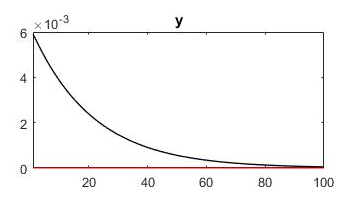
\includegraphics[width=0.4\linewidth]{y_2}
			\caption{}
			\label{fig:a1}
		\end{figure}
		\newpage
		\item \textbf{Imagen 3 y 4 (C y K):} Durante los primeros periodos posteriores al shock, tanto el consumo como el capital aumentan. Esto se debe a que mayor producto hace posible mayores niveles de consumo y hacen los factores más productivos. Posterior a esto, ambos bajan fuertemente conforme el shock vuelve a su estado natural, llegando a su estado estacionario en el largo plazo
		
	
		
		
		\item \textbf{Imagen 4 (I)}: La inversión, por su parte, aumenta en el periodo del shock por la misma razón que el capital (aumento en la productividad de los factores). Sin embargo, cae fuertemente conforme avanza el tiempo,  dado que cada vez el shock se acerca a su estado natural y a su vez hay cada vez más capital acumulado. Por esta misma razón, incluso hay un punto en que la inversión baja de su estado estacionario, con el propósito de converger al capital de estado estacionario.
	
		
		\item \textbf{(L y E)}: El esfuerzo experimenta un alza en el periodo inmediato del shock, dado que la productividad marginal aumenta. Sin embargo, vuelve rápidamente a su estado estacionario. Finalmente, el trabajo también sube pero sufre una caída más suave que el esfuerzo, incluso llegando por debajo de su estadio estacionario, para volver paulatinamente a su estado estacionario en el largo plazo.
		
	
		
	\end{itemize}

	\newpage
	\section{Pregunta 2}
	
	\subsection {a)}
	$$
	\max_{}
$$
Lagrangiano:
	$$
	\mathcal{L}:E_{0}\sum_{t}^\infty \beta^{t}{[\gamma ln c_{t} + \eta (1-e_{t}l_{t})-\dfrac{\kappa}{2}(e_{t}-1)^2l_{t}]+\lambda_{t}[A_t k_t^\alpha (e_tl_t)^{1-\alpha}+d_t-c_t-k_{t+1}+(1-\delta)k_t-d_{t-1}(1+r_{t-1}-\dfrac{\phi(k_{t+1}-k_t)^2}{2})]}	
	$$\\
CPO  \\
\begin{equation}
	\mathcal{L}_{c_{t}}: 
\frac{\gamma}{c_t}= \lambda_t
\end{equation}

\begin{equation}
	\mathcal{L}_{l_{t}}: 
		\eta e_t+\dfrac{\kappa}{2}(e_{t}-1)^2=\frac{\gamma (1-\alpha)}{c_t} \dfrac{y_t}{l_t}
\end{equation}

\begin{equation}
	\mathcal{L}_{d_{t}}: 
\frac{\gamma}{c_t}=\beta (1+r_t)E_t	\frac{\gamma}{c_{t+1}}
\end{equation}

\begin{equation}
	\mathcal{L}_{k_{t+1}}: 
	\frac{\gamma}{c_t}[1+\phi(k_{t+1}-k_t)]=\beta \frac{\gamma}{c_{t+1}}[\alpha \dfrac{y_{t+1}}{k_{t+1}}+(1-\alpha)+\phi(k_{t+1}-k_t)]
\end{equation}

\begin{equation}
	\mathcal{L}_{e_{t}}: 
	\eta l_t+\kappa(e_{t}-1)l_t=\frac{\gamma (1-\alpha)}{c_t} \dfrac{y_t}{l_t}
\end{equation}
	\subsection{b)}
	\begin{enumerate}
		
		\item Trade off \\
		El costo marginal de esforzarse se representa en la parte izquierda de la ecuación (5) es decir $\eta l_t+\kappa(e_{t}-1)l_t$ el cual se iguala al beneficio marginal del esfuerzo (reflejado en la producción) que corresponde a $\frac{\gamma (1-\alpha)}{c_t} \dfrac{y_t}{l_t}$.\\
		Un shock en $A_t$ aumenta la producción y por ende el beneficio marginal del esfuerzo y de las horas trabajadas.\\
		La CPO en $e_t$ es creciente en $e_t$, mientras que respecto a $l_t$ es constante. 		
		Los beneficios marginales son decrecientes en el nivel de esfuerzo y de horas trabajadas.
	\end{enumerate}

\newpage
	\subsection{c)}
			\begin{figure}[h!]
		\centering
		\includegraphics[width=0.7\linewidth]{captura 1}
		\end{figure}
*línea azul corresponde al modelo estándar, línea punteada roja es RBC-SOE.
\begin{enumerate}
\item[1] La primera gráfica corresponde al impacto del shock en la producción, donde se verifica que es mayor y más persistente en el caso del modelo estándar.

\item[2] La segunda imagen corresponde al efecto del shock en el consumo. Se aprecia en este caso que a pesar del mayor impacto que se verifica en el modelo estándar, el shock es mucho menos persistente en comparación con el modelo $RBC- SOE$ 
	
\item[3] La figura 3 visualiza los efectos del shock en la inversión, donde se verifica que ambos modelos tienen un comportamiento muy similar tanto en impacto como en persistencia.
 
\item[4] La imagen 4 corresponde al esfuerzo. Dado que en el modelo estándar no existe $e_t$, tenemos que ese valor es constante e igual a 0.

\item[5] En esta parte se verifica que el impacto del shock es bastante semejante entre los modelos, sin embargo se muestra más persistente en el modelo $RBC-SOE$. Esto se debe a que no se puede ajustar de forma inmediata $l_t$.

\item[6] En la última imagen se evidencia que el impacto del shock es mucho más fuerte en el modelo $RBC_SOE$ pero menos persistente que en el modelo estándar.

\newpage
	\section{Pregunta 3}
	\subsection {a)}
	
	Lagrangiano:
	$$
	\mathcal{L}:E_{0}\sum_{t}^\infty \beta^{t}\left\lbrace\dfrac{[c_{t} - \dfrac{h_{t}^\omega}{\omega}]^{1-\sigma}}{1-\sigma}-\lambda_{t}
	[c_t+k_{t+1}-(1-\delta)k_t+d_{t-1}(1+r_{t-1})+\dfrac{\phi(k_{t+1}-k_t)^2}{2})-g_t-A_t k_t^\alpha h_t^{1-\alpha}-d_t]\right\rbrace 
$$
	CPO  
	\begin{equation}
		\mathcal{L}_{c_{t}}: 
		(c_{t} - \dfrac{h_{t}^\omega}{\omega})^{-\sigma} = \lambda_t
	\end{equation}
	
	\begin{equation}
		\mathcal{L}_{h_{t}}: 
	(c_{t} - \dfrac{h_{t}^\omega}{\omega})^{-\sigma} h_t^{\omega-1} = \lambda_t (1-\alpha)A_t k_t^\alpha h_t^{-\alpha}
	\end{equation}
	
	\begin{equation}
		\mathcal{L}_{d_{t}}: 
		\lambda_t=\beta (1+r_t)E_t	\lambda_{t+1}
	\end{equation}
	
	\begin{equation}
		\mathcal{L}_{k_{t+1}}: 
		\lambda_{t}[1+\phi(k_{t+1}-k_t)]=\beta E_t \lambda_{t+1}[\alpha \dfrac{y_{t+1}}{k_{t+1}}+(1-\delta)+\phi(k_{t+1}-k_t)]
		\end{equation}
	
	\begin{equation}
		ln A_t=\rho_A \ln A_{t-1}+\varepsilon_{A,t}
	\end{equation}
	
	\begin{equation}
		g_t=\rho_g \ln g_{t-1}+\varepsilon_{g,t}
	\end{equation}

	
		\subsection {b)}
		steady state
		\begin{equation}
			A=1 		
		\end{equation}
		\begin{equation}
			g=0 
		\end{equation}
	    \begin{equation}
            d=\hat{d}
	    \end{equation}
		\begin{equation}
		r^*d=y-c-\delta k-g
		\end{equation}
		
		\begin{equation}
		h_t^{\omega-1} = (1-\alpha)A_t k_t^\alpha h_t^{-\alpha}
		\end{equation}
		
		\begin{equation}
			1 =\beta (1+r^*)
		\end{equation}
		
		\begin{equation}
			1 =\beta[\alpha \dfrac{y}{k}+(1-\delta)]
		\end{equation}

	
	
\end{enumerate}
	
\end{document}
